\documentclass[10pt,twocolumn,letterpaper]{article}

% Use official WACV template in Overleaf.
% For review: \usepackage[review,datasets]{wacv}
% If your author kit only provides cvpr.sty, replace wacv by cvpr.
\usepackage[review,datasets]{wacv}

\usepackage[utf8]{inputenc}
\usepackage{times}
\usepackage{epsfig}
\usepackage{graphicx}
\usepackage{amsmath,amssymb}
\usepackage{booktabs}
\usepackage{multirow}
\usepackage{xspace}
\usepackage{enumitem}
\usepackage{pifont}
\usepackage{color}
\usepackage{array}
\usepackage{makecell}
\usepackage{tabularx}
\usepackage[pagebackref,breaklinks,colorlinks]{hyperref}

\newcommand{\method}{FairRSFM\xspace}
\newcommand{\biobench}{\textsc{BiomeBench-RS}\xspace}
\newcommand{\bbal}{\textsc{Biome-Balanced ERM}\xspace}
\newcommand{\bdro}{\textsc{BiomeDRO}\xspace}
\newcommand{\redtodo}[1]{\textcolor{red}{[TODO: #1]}}
\newcommand{\cmark}{\ding{51}}
\newcommand{\xmark}{\ding{55}}

\def\wacvPaperID{2158}
\def\confName{WACV}
\def\confYear{2027}


\title{\method: A Biome-Aware Benchmark and Debiasing Framework for Remote Sensing Foundation Models}

% FairRSFM: A Biome-Aware Benchmark and Debiasing Framework for Remote Sensing Foundation Models

\author{Anonymous WACV Submission}

\begin{document}
\maketitle

\begin{abstract}
Remote sensing foundation models (RSFMs) are commonly evaluated using aggregate metrics, but such scores can hide systematic performance disparities across ecological regions. We introduce \method, a biome-aware benchmark and debiasing framework for studying ecological group robustness in RSFMs. \method maps georeferenced samples from 14 terrestrial biome classes into six ecologically meaningful biome macro-groups and evaluates models under a unified frozen-backbone linear-probing protocol. The benchmark covers four representative downstream datasets: m-EuroSAT for single-label land-cover classification, m-BigEarthNet for multi-label land-cover classification, m-SA-Crop-Type for crop-type segmentation, and MMEarth20K with Dynamic World label maps for dense land-cover segmentation. Using Prithvi-EO-2.0 as a case-study RSFM across these four datasets, we show that aggregate performance hides substantial biome-dependent disparities. For example, m-EuroSAT obtains only 0.800 macro-F1 in Boreal Forests/Taiga, while m-SA-Crop-Type ranges from 0.2891 mIoU in Mediterranean regions to 0.1755 in Deserts and Xeric Shrublands. To mitigate such disparities without updating the RSFM backbone, we propose Biome-Orthogonal Linear Probing (BOLP), which removes biome-associated directions from frozen embeddings before training the task head. BOLP improves the worst-group performance on m-EuroSAT from 83.72\% to 84.34\% and on m-BigEarthNet from 46.12\% to 50.27\%, while also reducing cross-biome disparity measures. These results show that biome-aware evaluation can reveal ecological disparities across classification and segmentation tasks, and that mitigation strategies like BOLP and GroupDRO can help reduce such disparities.

\end{abstract}



\section{Introduction}

Remote sensing foundation models (RSFMs) have shown strong transferability across diverse Earth-observation tasks, including land-cover classification, crop mapping, flood segmentation, and semantic segmentation. Large pretrained encoders such as SatMAE~\cite{satmae}, Prithvi-EO-2.0~\cite{prithvi2}, DOFA~\cite{dofa}, SpectralGPT~\cite{spectralgpt}, and related RSFMs are increasingly used as general-purpose backbones for downstream remote-sensing applications. Benchmark suites such as GEO-Bench~\cite{geobench} have accelerated this trend by providing classification and segmentation tasks for systematic evaluation of pretrained models.

However, most RSFM evaluations still report only aggregate dataset-level metrics such as accuracy, macro-F1, or mean intersection-over-union (mIoU). These aggregate metrics answer whether a model performs well \emph{on average}, but they do not reveal whether the model performs consistently across ecological regions. This is a critical issue for remote sensing because Earth-observation data are spatially and ecologically structured: the appearance of the same semantic class can change substantially across forests, grasslands, deserts, Mediterranean ecosystems, boreal regions, and agricultural landscapes. A model may therefore achieve high average accuracy while underperforming in specific ecological regions that are visually, climatically, or geographically under-represented. This omission matters in practice because geospatial models can degrade substantially under realistic natural distribution shifts, including geographic, sensor, scale, and source changes~\cite{rolf2023evaluation,earthshift2026}.


We focus on \textbf{biome bias}, which we define as systematic disparity in RSFM downstream performance across biome-derived ecological groups. A biome is a large ecological region characterized by similar climate, vegetation, and environmental conditions. To measure this bias, we assign each georeferenced sample to a biome label using its geographic coordinates and an external terrestrial ecoregion reference map~\cite{terrestrialecoregions,ecoregions2017}. We then evaluate model performance separately within each biome-derived group rather than only reporting a single aggregate dataset-level score. This converts standard RSFM transfer evaluation into a group-robustness problem, where poor worst-group performance can indicate representational bias of the foundation model in specific ecological regimes.

Although the reference taxonomy contains 14 terrestrial biome classes, directly using all 14 classes as fairness groups can be unstable for downstream datasets with limited or uneven biome coverage. We therefore adopt a two-level grouping strategy. Each sample is first mapped to one of the 14 raw terrestrial biome labels and then consolidated into six biome macro-groups reflecting broad spectral, phenological, hydrological, cryospheric, and surface-property regimes. These groups correspond to aseasonal high-biomass regions, high-amplitude phenological forests, transitional herbaceous and scrub landscapes, cryospheric and short-cycle regions, xeric and mineralogical surfaces, and hydrologically modulated ecosystems. This design preserves ecological interpretability while providing more reliable group-wise estimates for fairness evaluation and debiasing.

To address this gap, we introduce \method, a biome-aware benchmark and debiasing framework for evaluating ecological group robustness in remote sensing foundation models. Our benchmark design is inspired by GEO-Bench but differs in objective. GEO-Bench was designed to evaluate foundation models across a diverse set of Earth-monitoring tasks, including classification and segmentation datasets~\cite{geobench}. In contrast, \method uses three selected GEO-Bench tasks together with an MMEarth20K Dynamic World segmentation subset to ask a different question: \emph{Do RSFMs generalize fairly across biome-derived ecological groups?} This question is particularly important for global Earth-observation deployment, where a model trained or evaluated mostly on dominant ecological regimes may fail in less represented regions.

Beyond diagnosis, \method also includes a biome-aware debiasing framework under the same frozen-backbone linear-probing protocol. We use biome-balanced ERM as a simple mitigation baseline and define stronger biome-aware strategies, including  Dynamic Biome Reweighting with Validation Feedback (DBR), and Biome-Orthogonal Linear Probing (BOLP). BOLP removes biome-associated directions from frozen RSFM embeddings before training the task head, providing a representation-level debiasing strategy. This allows us to analyze whether biome-dependent disparities can be reduced without full backbone fine-tuning.

Our main contributions are as follows:
\begin{itemize}[leftmargin=*]
    \item We introduce \method, a biome-aware benchmark and debiasing framework for studying ecological group robustness in remote sensing foundation models across four classification and segmentation datasets.

    \item We propose a biome-labeling pipeline that first assigns georeferenced samples to the 14 terrestrial biome classes and then groups them into six biome macro-groups reflecting spectral, phenological, hydrological, cryospheric, and surface-property regimes.

    \item We evaluate Prithvi-EO-2.0 using a unified frozen-backbone linear-probing protocol and report both standard task metrics and biome-aware robustness measures, showing that strong aggregate performance can hide substantial biome-dependent disparities.
        
    \item We develop a set of biome-aware mitigation strategies, including Dynamic Biome Reweighting with Validation Feedback (DBR), and Biome-Orthogonal Linear Probing (BOLP), and empirically evaluate BOLP as our main representation-level debiasing method.
\end{itemize}

\section{Related Work}

\noindent\textbf{Remote sensing foundation models.} RSFMs learn transferable representations from large-scale Earth observation via self-supervised pretraining on multispectral, temporal, and multimodal imagery~\cite{rsfm_survey_multimodal}. These span masked-autoencoding models such as SatMAE~\cite{satmae}, Scale-MAE~\cite{scalemae}, and SatMAE++~\cite{satmaepp}; contrastive and hybrid objectives such as CROMA~\cite{croma} and SoftCon~\cite{softcon}; and recent broad-coverage models including Prithvi-EO-2.0~\cite{prithvi2}, DOFA~\cite{dofa}, SpectralGPT~\cite{spectralgpt}, and SkySense~\cite{skysense}. These models are commonly evaluated with aggregate metrics such as accuracy, macro-F1, or mIoU, which cannot reveal whether performance holds consistently across ecological regions; \method targets this gap.

\smallskip
\noindent\textbf{Remote sensing benchmarks.} Standardized suites have driven RSFM evaluation: GEO-Bench~\cite{geobench} provides harmonized classification and segmentation tasks, from which we use m-EuroSAT, m-BigEarthNet, and m-SA-Crop-Type; we further include MMEarth20K, a subset of MMEarth~\cite{mmearth} with Dynamic World~\cite{dynamicworld} label maps, to increase dense land-cover segmentation coverage. PANGAEA~\cite{pangaea} broadens geospatial foundation-model evaluation across tasks, resolutions, and geographies. Widely used operational datasets include BigEarthNet~\cite{bigearthnet,bigearthnetmm}, MMEarth~\cite{mmearth}, and Dynamic World~\cite{dynamicworld}. Recent work has quantified remote-sensing dataset bias through size, angle, class, density, and scene factors using diversity- and evenness-based indices~\cite{rsd_biaseval}. Existing benchmarks usually summarize each dataset with a single aggregate score and do not test whether performance holds across ecological regions within the dataset. \method reuses this ecosystem for a complementary purpose: measuring how RSFM performance varies across biome-derived groups.

\smallskip
\noindent\textbf{Fairness, group robustness, and representation debiasing.} Fairness evaluation compares behavior across groups rather than population-level averages~\cite{fairnesssurvey}, since a model can score well on average yet fail on under-represented groups, motivating worst-group and GroupDRO-style objectives~\cite{groupdro,wilds}. These concerns are acute in remote sensing, yet the field lacks a domain-appropriate notion of groups; we use biomes because they are globally defined, ecologically meaningful, and tightly tied to land-cover appearance, climate, and surface conditions. In this sense, biome groups act as ecologically meaningful analysis groups for subgroup-error evaluation under distribution shift~\cite{hardt2016equality,woodworth2017learning,shao2024fairnessshift}. Bias mitigation for RSFMs remains nascent, limited to parameter-efficient tuning~\cite{yin2025remote} and LoRA-based debiasing under long-tailed data (debLoRA)~\cite{deblora}, while more general representation debiasing removes attribute-associated directions from embeddings~\cite{bolukbasi2016man,ravfogel2020null}. Our Biome-Orthogonal Linear Probing (BOLP) brings this idea to ecological bias, removing biome directions from frozen embeddings in closed form without backbone fine-tuning or adapters.


\begin{figure*}
    \centering
    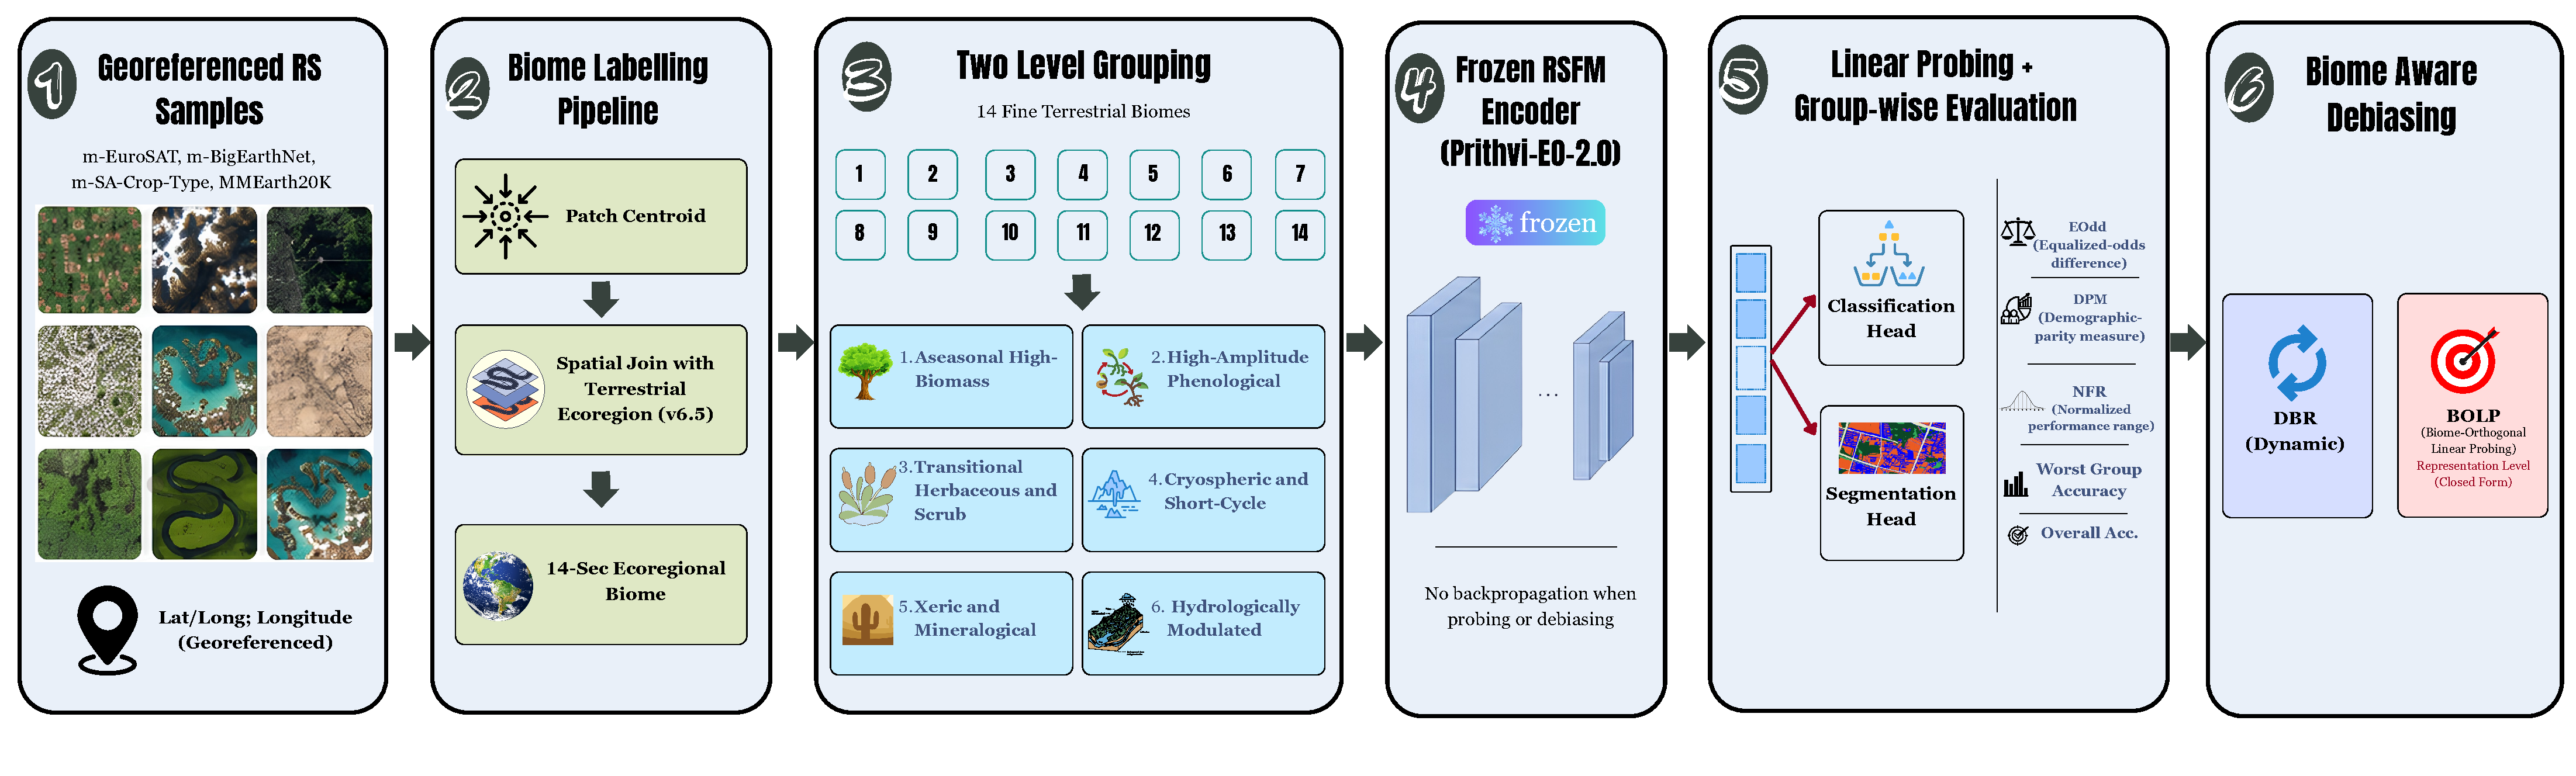
\includegraphics[width=0.95\linewidth]{model.pdf}
    % \caption{Overview of the \method benchmark and debiasing framework. Georeferenced samples are first mapped from 14 terrestrial biome classes to six ecologically meaningful macro-groups. A frozen RSFM backbone produces embeddings that are evaluated under a unified linear-probing protocol on classification and segmentation tasks. Biome-Orthogonal Linear Probing (BOLP) removes biome-associated directions from the frozen features before training the task head. Both standard task metrics and group-robustness measures (worst-group performance, normalized performance range, equalized odds difference, etc.) are reported to diagnose and mitigate ecological disparities.}
    \caption{Overview of \method. Georeferenced samples are mapped from 14 terrestrial biomes to six macro-groups and evaluated under a frozen-backbone linear-probing protocol. Biome-Orthogonal Linear Probing (BOLP) removes biome-associated directions from RSFM embeddings before training the task head.}
    \label{fig:main}
\end{figure*}

\section{FairRSFM Benchmark}

\subsection{Task Families and Datasets}

\method contains two application families: \textbf{classification} and \textbf{semantic segmentation}. Classification tasks evaluate whether frozen RSFM features are discriminative for patch-level labels, while segmentation tasks evaluate whether RSFM representations support dense prediction under biome-derived ecological variation. Table~\ref{tab:datasets} summarizes the four-dataset benchmark suite. We use three GEO-Bench tasks covering single-label classification, multi-label classification, and crop-type segmentation, and add an MMEarth20K subset with Dynamic World label maps to increase dense land-cover segmentation diversity.

\begin{table*}[t]
\centering
\caption{\method dataset suite. GEO-Bench datasets are selected for classification and segmentation; the MMEarth20K subset increases dense land-cover segmentation diversity. Sample counts for GEO-Bench tasks follow the modified benchmark setting.}
\label{tab:datasets}
\scalebox{0.9}{
\begin{tabular}{l l c c c c l}
\toprule
Dataset & Task & Classes & Train & Val & Test & Notes \\
\midrule
m-EuroSAT~\cite{geobench} & Classification & 10 & 2,000 & 1,000 & 1,000 & Sentinel-2, land cover \\
m-BigEarthNet~\cite{geobench,bigearthnet} & Multi-label classification & 43 & 20,000 & 1,000 & 1,000 & Sentinel-2, multi-label land cover \\
m-SA-Crop-Type~\cite{geobench} & Segmentation & 10 & 3,000 & 1,000 & 1,000 & Sentinel-2, crop type \\
MMEarth20K~\cite{mmearth,dynamicworld} & Segmentation & 9 & 16,000 & 2,000 & 2,000 & Dynamic World label maps \\
\bottomrule
\end{tabular}
}
\end{table*}

For MMEarth20K, we use a 20,000-sample subset with Dynamic World-derived 10\,m land-cover label maps. The subset is split into 16,000 training samples, 2,000 validation samples, and 2,000 test samples, enabling biome-aware dense land-cover evaluation under the same frozen-backbone protocol.

\begin{figure}[h]
    \centering
    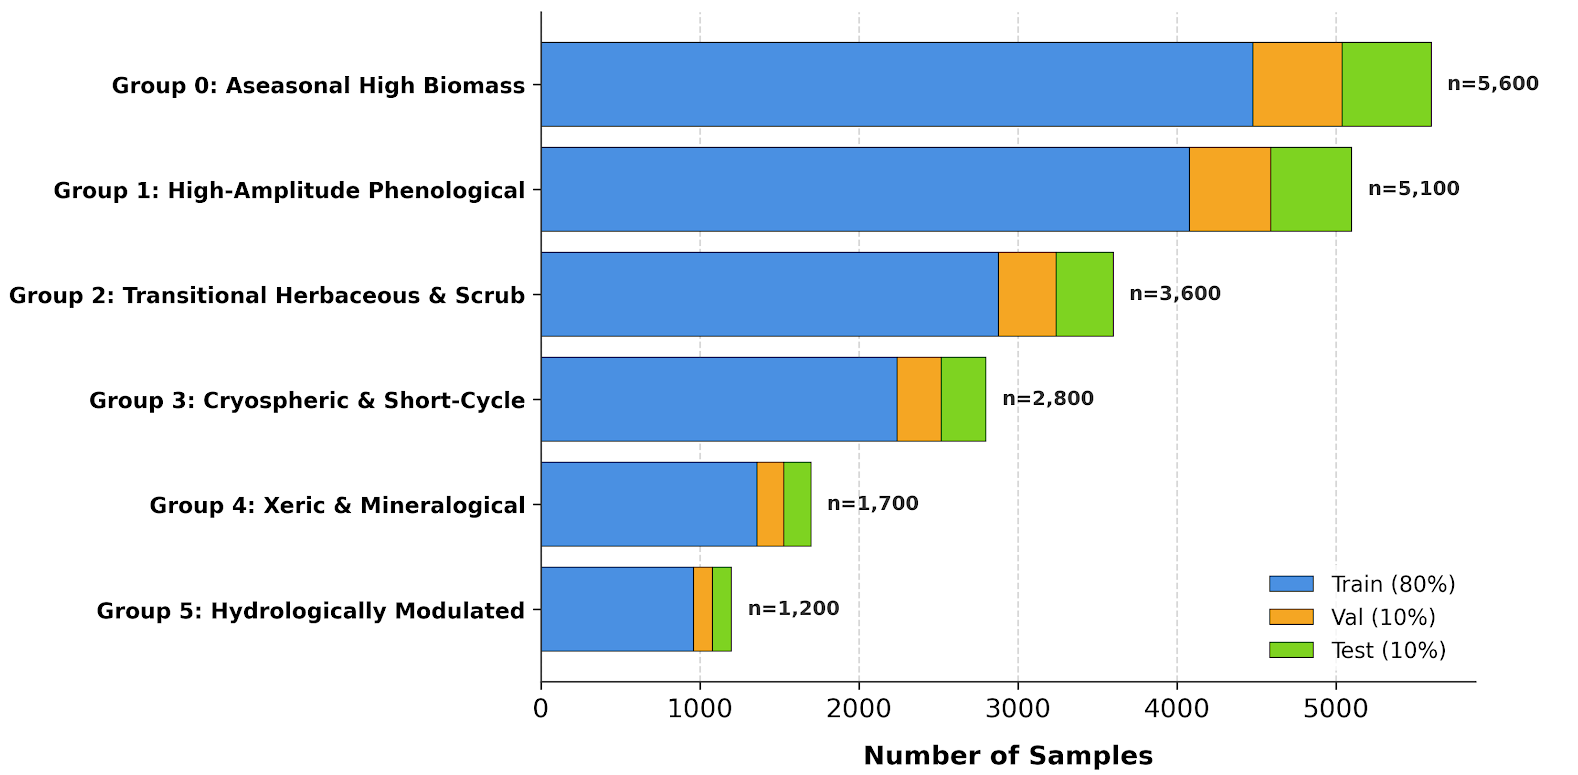
\includegraphics[width=\linewidth]{macro_group_distribution.png}
    \caption{Quantitative sample distribution of the curated MMEarth20K subset across six macro ecological groups and corresponding data splits (80\% Train, 10\% Val, 10\% Test).}
    \label{fig:macro_group_dist}
\end{figure}

\subsection{Biome Label Construction}
The central grouping variable in \method is derived from terrestrial biome information. We use the 14-biome taxonomy from global terrestrial ecoregion products~\cite{terrestrialecoregions,ecoregions2017}. For each georeferenced sample, we compute the patch centroid and spatially join it with an external biome reference map. The resulting raw biome ID is stored as image-level metadata. For segmentation datasets, the entire patch is assigned a biome label based on its centroid, which keeps the grouping protocol consistent across classification and dense prediction tasks.

Directly using all 14 raw biome classes as fairness groups can be unstable for downstream datasets with limited or uneven biome coverage. Therefore, \method uses a two-level grouping strategy. Each sample is first assigned a raw biome label \(b_i\in\{1,\ldots,14\}\), and the raw label is then mapped to a biome macro-group \(g_i\in\{1,\ldots,6\}\). The six macro-groups are designed to reflect broad spectral, phenological, hydrological, cryospheric, and surface-property regimes. They are used as the primary groups for fairness evaluation and debiasing, while the original 14 biome labels are retained for fine-grained analysis when sufficient samples are available.

% \begin{table*}[t]
% \centering
% \caption{Mapping from 14 terrestrial biome classes to six biome macro-groups used for primary fairness evaluation and debiasing in \method.}
% \label{tab:biome_macro_groups}
% \resizebox{\textwidth}{!}{
% \begin{tabular}{c l l l}
% \toprule
% Group ID & Biome macro-group & Included raw biome classes & Rationale \\
% \midrule
% 1 & Aseasonal High-Biomass &
% 1 Tropical Moist Forests; 3 Tropical Conifer Forests; 5 Temperate Conifer Forests &
% Dense, high-biomass vegetation with relatively persistent canopy structure. \\

% 2 & High-Amplitude Phenological &
% 2 Tropical Dry Forests; 4 Temperate Broadleaf and Mixed Forests; 6 Boreal Forests/Taiga &
% Forested regions with strong seasonal or phenological variation. \\

% 3 & Transitional Herbaceous and Scrub &
% 7 Tropical and Subtropical Grasslands, Savannas and Shrublands; 8 Temperate Grasslands, Savannas and Shrublands; 12 Mediterranean Forests, Woodlands and Scrub &
% Open or mixed vegetation regimes with strong grass, shrub, soil, and canopy heterogeneity. \\

% 4 & Cryospheric and Short-Cycle &
% 10 Montane Grasslands and Shrublands; 11 Tundra &
% Temperature-restricted ecosystems with short growing periods or cryospheric influence. \\

% 5 & Xeric and Mineralogical &
% 13 Deserts and Xeric Shrublands &
% Vegetation-sparse surfaces dominated by albedo, exposed soil, and mineral background. \\

% 6 & Hydrologically Modulated &
% 9 Flooded Grasslands and Savannas; 14 Mangroves &
% Water-influenced ecosystems where inundation strongly affects spectral response. \\
% \bottomrule
% \end{tabular}}
% \end{table*}

\begin{table*}[t]
\centering 
\footnotesize
% \setlength{\tabcolsep}{5pt}
% \renewcommand{\arraystretch}{1.15}
% \scalebox{0.8}{
\caption{Mapping from 14 terrestrial biome classes to six biome macro-groups used for primary fairness evaluation and debiasing in \method.}
\label{tab:biome_macro_groups}
\begin{tabularx}{\textwidth}{@{} c l
  >{\hsize=1.14\hsize\raggedright\arraybackslash}X
  >{\hsize=0.86\hsize\raggedright\arraybackslash}X @{}}
\toprule
\textbf{ID} & \textbf{Biome macro-group} & \textbf{Included raw biome classes} & \textbf{Rationale} \\
\midrule
1 & Aseasonal High-Biomass &
1 Tropical Moist Forests; 3 Tropical Conifer Forests; 5 Temperate Conifer Forests &
Dense, high-biomass vegetation with relatively persistent canopy structure. \\
\addlinespace[2pt]
2 & High-Amplitude Phenological &
2 Tropical Dry Forests; 4 Temperate Broadleaf and Mixed Forests; 6 Boreal Forests/Taiga &
Forested regions with strong seasonal or phenological variation. \\
\addlinespace[2pt]
3 & Transitional Herbaceous and Scrub &
7 Tropical and Subtropical Grasslands, Savannas and Shrublands; 8 Temperate Grasslands, Savannas and Shrublands; 12 Mediterranean Forests, Woodlands and Scrub &
Open or mixed vegetation regimes with strong grass, shrub, soil, and canopy heterogeneity. \\
\addlinespace[2pt]
4 & Cryospheric and Short-Cycle &
10 Montane Grasslands and Shrublands; 11 Tundra &
Temperature-restricted ecosystems with short growing periods or cryospheric influence. \\
\addlinespace[2pt]
5 & Xeric and Mineralogical &
13 Deserts and Xeric Shrublands &
Vegetation-sparse surfaces dominated by albedo, exposed soil, and mineral background. \\
\addlinespace[2pt]
6 & Hydrologically Modulated &
9 Flooded Grasslands and Savannas; 14 Mangroves &
Water-influenced ecosystems where inundation strongly affects spectral response. \\
\bottomrule
\end{tabularx}
% }
\end{table*}


% \begin{figure}
%     \centering
%     \includegraphics[width=1\linewidth]{Construction.pdf}
%     \caption{Enter Caption}
%     \label{fig:placeholder}
% \end{figure}

Unknown, water-only, or unmatched samples are reported separately and are not used for the primary worst-group score unless explicitly stated. Some datasets cover only a subset of the six macro-groups, and therefore all fairness metrics are computed over the set of matched macro-groups present in each dataset split.

% \vspace{-0.5em}

\subsection{Biome Metadata Schema}

Each sample is associated with the following metadata: $(x_i, y_i, d_i, \ell_i, b_i, g_i),$ where \(x_i\) is the input image, \(y_i\) is the class label or segmentation mask, \(d_i\) is the dataset name, \(\ell_i=(\mathrm{lat}_i,\mathrm{lon}_i)\) is the sample location, \(b_i\in\{1,\ldots,14\}\) is the raw terrestrial biome label, and \(g_i\in\{1,\ldots,6\}\) is the derived biome macro-group label. The macro-group is obtained through a deterministic mapping \(g_i=\psi(b_i)\), where \(\psi\) is defined in Table~\ref{tab:biome_macro_groups}. For single-label classification, \(y_i\in\{1,\ldots,C\}\); for multi-label classification, \(y_i\in\{0,1\}^{C}\); and for segmentation, \(y_i \in \{1,\ldots,C\}^{H\times W}\).

The raw biome label \(b_i\) enables fine-grained ecological analysis, while the macro-group label \(g_i\) is used for the primary fairness metrics and mitigation methods. This separation allows \method to preserve ecological detail without making the primary robustness analysis overly sensitive to sparse biome classes.

% \subsection{Evaluation Metrics}

% Let \(\mathcal{G}_d\) denote the set of matched biome macro-groups present in dataset \(d\), and let \(M_g\) be the task-specific metric computed on macro-group \(g\). Unless otherwise stated, all group-wise fairness metrics are computed over \(\mathcal{G}_d\). Raw 14-biome results can also be reported as a fine-grained diagnostic when enough samples are available.

% \textbf{Classification.} For single-label classification, we report macro-F1 and balanced accuracy. For multi-label classification such as m-BigEarthNet, we report macro-F1 at per-class optimal thresholds, denoted F1@opt, and mAP where available. Group-wise macro-F1 is computed over samples belonging to each biome macro-group. When necessary, per-group macro-F1 is computed only over classes present in that group to avoid penalizing an ecological group for naturally absent land-cover categories.

% \textbf{Segmentation.} For segmentation, we report global mIoU and group-wise mIoU. Each image patch is assigned to a biome macro-group using its centroid. For each macro-group \(g\),
% \begin{equation}
% \mathrm{mIoU}_g = \frac{1}{C_g}\sum_{c\in C_g}\frac{\mathrm{TP}_{g,c}}{\mathrm{TP}_{g,c}+\mathrm{FP}_{g,c}+\mathrm{FN}_{g,c}},
% \end{equation}
% where \(C_g\) is the set of classes present in macro-group \(g\).

% \textbf{Worst-group metric.}
% \begin{equation}
% M_{\mathrm{worst}} = \min_{g\in\mathcal{G}_d} M_g.
% \end{equation}

% \textbf{Normalized performance range.}
% \begin{equation}
% \mathrm{NFR}=\frac{\max_{g\in\mathcal{G}_d}M_g-\min_{g\in\mathcal{G}_d}M_g}{\frac{1}{|\mathcal{G}_d|}\sum_{g\in\mathcal{G}_d}M_g+\epsilon}.
% \end{equation}

% \textbf{Group standard deviation.}
% \begin{equation}
% \sigma_{\mathrm{group}} = \sqrt{\frac{1}{|\mathcal{G}_d|}\sum_{g\in\mathcal{G}_d}\left(M_g-\bar{M}\right)^2},
% \end{equation}
% where \(\bar{M}=\frac{1}{|\mathcal{G}_d|}\sum_{g\in\mathcal{G}_d}M_g\).

% \textbf{Equalized odds difference.} For classification, we compute one-vs-rest TPR and FPR for each class and compare them across macro-group pairs:
% \begin{equation}
% \mathrm{EOdd}=\max_{g,g',c}\frac{1}{2}\left(|\mathrm{TPR}_{g,c}-\mathrm{TPR}_{g',c}|+|\mathrm{FPR}_{g,c}-\mathrm{FPR}_{g',c}|\right).
% \end{equation}

% \textbf{Demographic parity measure.} DPM measures the maximum cross-group prediction-rate difference. For single-label classification, \(\hat{y}_c\) denotes the indicator that class \(c\) is predicted; for multi-label classification, it denotes the predicted positive indicator for class \(c\):
% \begin{equation}
% \mathrm{DPM}=\max_{g,g',c}\left|P(\hat{y}_c=1\mid g)-P(\hat{y}_c=1\mid g')\right|.
% \end{equation}

\subsection{Evaluation Metrics}
Let $\mathcal{G}_d$ be the set of active biome macro-groups present in dataset $d$ ($K = |\mathcal{G}_d|$), and let $M_g$ denote the task-specific metric evaluated on group $g \in \mathcal{G}_d$. To comprehensively diagnose ecological robustness, calibration, and subgroup parity, \method evaluates models across three complementary metric tiers:

\smallskip
\noindent\textbf{1. Per-Task Performance Metrics.}
For single-label classification (m-EuroSAT), we report macro-F1 over present classes $C_g$: $\mathrm{Macro\text{-}F1}_g = \frac{1}{|C_g|}\sum_{c\in C_g}\mathrm{F1}_{g,c}$. For multi-label classification (m-BigEarthNet), we report macro-F1 at per-class optimal validation thresholds $\tau_c \in [0.1, 0.95]$, denoted $\mathrm{F1@opt}_g = \frac{1}{|C_g|}\sum_{c\in C_g}\mathrm{F1}_{g,c}(\tau_c)$. For segmentation (m-SA-Crop-Type, MMEarth20K), we report group-wise mean Intersection-over-Union:
\begin{equation}
\mathrm{mIoU}_g = \frac{1}{|C_g|}\sum_{c\in C_g}\frac{\mathrm{TP}_{g,c}}{\mathrm{TP}_{g,c}+\mathrm{FP}_{g,c}+\mathrm{FN}_{g,c}}.
\end{equation}

\smallskip
\noindent\textbf{2. Group Disparity \& Robustness Summaries.}
From the set of group performance scores $\{M_g\}_{g\in\mathcal{G}_d}$ and group mean $\bar{M} = \frac{1}{K}\sum_{g} M_g$:
\begin{itemize}[leftmargin=*]
    \item \textbf{Worst-Group Score ($M_{\mathrm{worst}}$):} $M_{\mathrm{worst}} = \min_{g\in\mathcal{G}_d} M_g$.
    \item \textbf{Normalized Failure Range ($\mathrm{NFR} \downarrow$):} Relative spread normalized by the mean score, $\mathrm{NFR} = \frac{\max_g M_g - \min_g M_g}{\bar{M} + \epsilon}$.
\end{itemize}

\smallskip
\noindent\textbf{3. Calibration \& Fairness Disparity Metrics.}
\begin{itemize}[leftmargin=*]
    \item \textbf{Expected Calibration Error ($\mathrm{ECE} \downarrow$):} Model confidence scores are partitioned into $B=10$ equal-width bins $\{B_m\}_{m=1}^B$:
    \begin{equation}
    \mathrm{ECE} = \sum_{m=1}^B \frac{|B_m|}{N} \left| \mathrm{acc}(B_m) - \mathrm{conf}(B_m) \right|.
    \end{equation}
    \item \textbf{Equalized Odds Disparity ($\mathrm{EOdd} \downarrow$):} Evaluates error-rate balance across groups via Youden's $J$-index $J_{g,c} = \mathrm{TPR}_{g,c} - \mathrm{FPR}_{g,c}$. The metric measures the maximum cross-group disparity averaged across classes:
    \begin{equation}
    \mathrm{EOdd} = \max_{g, g' \in \mathcal{G}_d} \frac{1}{|C|} \sum_{c \in C} \left| J_{g,c} - J_{g',c} \right|.
    \end{equation}
    \item \textbf{Demographic Parity Metric ($\mathrm{DPM} \downarrow$):} Quantifies disparities in positive prediction rates $\mathrm{PPR}_{g,c} = P(\hat{y}_c = 1 \mid g)$ between ecological strata:
    \begin{equation}
    \mathrm{DPM} = \max_{g, g' \in \mathcal{G}_d} \frac{1}{|C|} \sum_{c \in C} \left| \mathrm{PPR}_{g,c} - \mathrm{PPR}_{g',c} \right|.
    \end{equation}
\end{itemize}


% \section{Biome-Aware Debiasing Framework}

% Let $\mathcal{D}_{\mathrm{tr}}=\{(x_i,y_i,g_i)\}_{i=1}^{N}$ be the training set with input image $x_i$, task label $y_i$, and biome macro-group label $g_i\in\mathcal{G}$ (Table~\ref{tab:biome_macro_groups}). Let $\phi:X\rightarrow\mathbb{R}^{d}$ be a frozen RSFM encoder and $z_i=\phi(x_i)$ the frozen representation. Every strategy below keeps $\phi$ fixed and trains only the downstream head $h_\theta$, so any change in fairness or robustness is attributable to the mitigation rather than to backbone fine-tuning. The task loss $\ell$ is cross-entropy for single-label classification, binary cross-entropy for multi-label classification, and a pixel- or decoder-level loss for segmentation.

% \begin{equation}
% w_g=\frac{1/p_g}{\frac{1}{|\mathcal{G}|}\sum_{g'\in\mathcal{G}}1/p_{g'}}\label{eq:wg}
% \end{equation}

% \subsection{Dynamic Biome Reweighting with Validation Feedback}
% Static weights are fixed from the training distribution, yet the most under-represented group is not always the worst-performing one during training. Dynamic Biome Reweighting (DBR) therefore initializes $w^{(0)}_g$ to the static weights of Eq.~\eqref{eq:wg} and adapts them from validation feedback. Every $K$ epochs the current model is evaluated per group; let $M_g^{(t)}$ be the group-$g$ validation metric at update step $t$ (macro-F1 for classification, mIoU for segmentation) and $\bar{M}^{(t)}=\frac{1}{|\mathcal{G}|}\sum_{g}M_g^{(t)}$ its mean. DBR raises the weight of below-mean groups and lowers it for above-mean groups, then renormalizes to unit average:
% \begin{align}
% \tilde{w}^{(t+1)}_g&=w^{(t)}_g\!\left(1+\alpha\,\frac{\bar{M}^{(t)}-M_g^{(t)}}{\bar{M}^{(t)}+\epsilon}\right),\\
% w^{(t+1)}_g&=\frac{\tilde{w}^{(t+1)}_g}{\frac{1}{|\mathcal{G}|}\sum_{g'}\tilde{w}^{(t+1)}_{g'}}.
% \end{align}
% Here, $\alpha$ controls feedback strength and $\epsilon$ ensures numerical stability. The objective reuses the reweighted form with the current weights, $\mathcal{L}_{\mathrm{DBR}}=\frac{1}{N}\sum_{i}w^{(t)}_{g_i}\,\ell(h_\theta(\phi(x_i)),y_i)$. DBR maintains only a small dictionary of group weights, reuses validation metrics already computed for fairness evaluation, and is non-adversarial, parameter-free, and applicable to single-label, multi-label, and segmentation tasks.
\section{Biome-Aware Debiasing Framework}

Let \(\mathcal{D}_{\mathrm{tr}}=\{(x_i,y_i,g_i)\}_{i=1}^{N}\) be the training set with input image \(x_i\), task label \(y_i\), and biome macro-group label \(g_i\in\mathcal{G}\) (Table~\ref{tab:biome_macro_groups}). Let \(\phi:X\rightarrow\mathbb{R}^{d}\) be a frozen RSFM encoder and \(z_i=\phi(x_i)\) the frozen representation. Every strategy below keeps \(\phi\) fixed and trains only the downstream head \(h_\theta\), so any change in fairness or robustness is attributable to the mitigation rather than to backbone fine-tuning. The task loss \(\ell\) is cross-entropy for single-label classification, binary cross-entropy for multi-label classification, and a pixel- or decoder-level loss for segmentation.

\subsection{Dynamic Biome Reweighting with Validation Feedback}

We use Dynamic Biome Reweighting with Validation Feedback (DBR) as our loss-level mitigation strategy. DBR initializes group weights from a static inverse-frequency scheme and then adapts them dynamically during training according to per-group validation performance.

Let \(p_g = n_g / N\) be the empirical frequency of biome macro-group \(g\). DBR initializes the normalized weights as
\begin{equation}
w_g^{(0)}=\frac{1/p_g}{\frac{1}{|\mathcal{G}|}\sum_{g'\in\mathcal{G}}1/p_{g'}}\label{eq:wg}.
\end{equation}

Static weights alone are fixed from the training distribution, yet the most under-represented group is not always the worst-performing one. Therefore, every \(K\) epochs the current model is evaluated separately on each biome macro-group. Let \(M_g^{(t)}\) be the validation metric for group \(g\) at update step \(t\) (macro-F1 for classification, mIoU for segmentation) and \(\bar{M}^{(t)}=\frac{1}{|\mathcal{G}|}\sum_g M_g^{(t)}\) its mean. DBR increases the weight of groups performing below the mean and decreases it for groups performing above the mean, then renormalizes to preserve unit average:
\begin{align}
\tilde{w}^{(t+1)}_g &= w^{(t)}_g \left(1 + \alpha \frac{\bar{M}^{(t)} - M_g^{(t)}}{\bar{M}^{(t)} + \epsilon}\right), \\
w^{(t+1)}_g &= \frac{\tilde{w}^{(t+1)}_g}{\frac{1}{|\mathcal{G}|}\sum_{g'} \tilde{w}^{(t+1)}_{g'}}.
\end{align}
Here, \(\alpha\) controls feedback strength and \(\epsilon\) ensures numerical stability. The training objective reuses the current weights:
\begin{equation}
\mathcal{L}_{\mathrm{DBR}} = \frac{1}{N} \sum_{i=1}^N w^{(t)}_{g_i} \, \ell(h_\theta(\phi(x_i)), y_i).
\end{equation}
DBR is lightweight, reuses validation metrics already computed for fairness evaluation, is non-adversarial and parameter-free, and applies to single-label classification, multi-label classification, and segmentation tasks.

\subsection{Biome-Orthogonal Linear Probing}
Biome-Orthogonal Linear Probing (BOLP), our main representation-level method, acts on the geometry of the frozen embeddings rather than the loss. It is a closed-form module inserted between the frozen encoder and the linear head that removes biome-associated directions while preserving task-relevant variance.

\textbf{Precomputation.} For each group we form the centroid $\mu_g=\frac{1}{n_g}\sum_{i:g_i=g}z_i$, their mean $\mu_0=\frac{1}{|\mathcal{G}|}\sum_{g}\mu_g$, and the centered group-mean matrix
\begin{equation}
B=\left[\mu_{1}-\mu_{0},\;\ldots,\;\mu_{|\mathcal{G}|}-\mu_{0}\right]\in\mathbb{R}^{d\times|\mathcal{G}|}.
\end{equation}
From the thin SVD $B=U\Sigma V^{\top}$, the top $k$ left singular vectors $U_k\in\mathbb{R}^{d\times k}$ span the dominant inter-group mean-difference directions. Because the columns of $B$ sum to zero, at most $|\mathcal{G}|-1$ directions are non-trivial; hence, $k\le|\mathcal{G}|-1$. The projector onto their orthogonal complement is $P_k=I_d-U_kU_k^{\top}$. The buffers $\{\mu_g\}$, $\mu_0$, and $P_k$ are computed once on the training set and frozen.

\textbf{Debiasing transform.} For a sample with group label $g_i$, BOLP removes the first-order group-mean shift and projects out the biome-discriminative subspace,
\begin{equation}
\hat{z}_i=P_k\big(z_i-\mu_{g_i}+\mu_0\big),
\end{equation}
so $\hat{z}_i$ is recentered to a common reference (preserving the global feature scale) and lies in the orthogonal complement of the top inter-group mean-difference subspace.

\textbf{Linear probing.} The head is trained with the standard linear-probing objective on the debiased features, $\mathcal{L}_{\mathrm{BOLP}}=\frac{1}{N}\sum_{i}\ell(h_\theta(\hat{z}_i),y_i)$, with only $\theta$ trainable. At inference the same transform is applied when the group label is available; in georeferenced remote-sensing evaluation, this label can be obtained from the same coordinate-to-biome lookup used during preprocessing. If the group label is missing, the residualization is skipped and the global projector $P_k$ is still applied. BOLP adapts representation-debiasing and null-space projection~\cite{bolukbasi2016man,ravfogel2020null} to ecological group bias in frozen remote-sensing embeddings; unlike adapter- or LoRA-based mitigation it adds no trainable parameters and leaves the RSFM backbone unchanged.

\smallskip
\noindent\textbf{Method Comparison}
The two primary mitigation strategies evaluated in this work intervene at different stages of the frozen-backbone linear-probing pipeline. DBR operates at the loss level, dynamically adjusting biome macro-group weights each validation epoch based on per-group performance feedback. BOLP performs representation-level debiasing directly in the frozen embedding space: it first recenters each sample to remove group-mean shifts and then projects out the dominant inter-group directions via a closed-form null-space projection. Both methods retain the full training set and introduce no extra trainable parameters beyond the task head.



\section{Experiments}

\noindent \textbf{Experimental Protocol and Pretrained Baselines.}
To evaluate ecological robustness across diverse remote sensing representation paradigms, we benchmark three foundational architectures using their official pretraining configurations and checkpoints:
(i)~\textbf{Prithvi-EO-2.0}~\cite{prithvi2} (300M spatio-temporal ViT) using its official 6-band HLS configuration and channel statistics;
(ii)~\textbf{SatMAE}~\cite{satmae} (ViT-Large, 304M parameters) using its official 10 Sentinel-2 bands and pretraining statistics; and
(iii)~\textbf{DOFA}~\cite{dofa} (ViT-Base, 86M parameters) with dynamic continuous wavelength-conditioned positional embeddings ($0.44\mu\text{m}\text{--}2.20\mu\text{m}$).
Dataset splits and task definitions strictly follow \textbf{GEO-Bench}~\cite{geobench} (m-EuroSAT, m-BigEarthNet, m-SA-Crop-Type) and \textbf{MMEarth}~\cite{mmearth} (MMEarth20K).

\smallskip
\noindent \textbf{Controlled Frozen-Encoder Evaluation.}
In contrast to the original model papers that frequently fine-tuned backbones end-to-end for dense prediction (e.g., in DOFA~\cite{dofa} and SatMAE~\cite{satmae}), \method enforces a \textbf{strictly frozen encoder} $\phi(x)$ across all classification and dense segmentation tasks. Backpropagation updates only the task-specific linear/MLP head (for classification) or lightweight multi-level decoder (UPerNet/FCN for segmentation). This isolates representation quality and ensures that subgroup equity gains are strictly attributable to the mitigation strategy (ERM, BOLP, DBR, GroupDRO) rather than backbone gradient updates.

\smallskip
\noindent \textbf{Training and Optimization Details.}
Table~\ref{tab:training_config} summarizes the experimental configurations. All models are trained on $224\times224$ inputs using AdamW ($\beta_1=0.9, \beta_2=0.999$, base $\text{lr}=10^{-3}$ with cosine annealing down to $10^{-6}$, weight decay $10^{-4}$) for 50 epochs. All experiments are evaluated across $S=3$ independent random seeds. Checkpoints are selected on validation overall metric, and test subgroup performance ($M_{\mathrm{worst}}$, ECE, NFR, EOdd, DPM) is reported.

\begin{table}[t]
\centering
\caption{Unified benchmarking configurations across foundation models.}
\label{tab:training_config}
\setlength{\tabcolsep}{2.5pt}
\renewcommand{\arraystretch}{1.05}
\scriptsize
\resizebox{\linewidth}{!}{%
\begin{tabular}{lccc}
\toprule
\textbf{Configuration} & \textbf{Prithvi-EO-2.0}~\cite{prithvi2} & \textbf{SatMAE}~\cite{satmae} & \textbf{DOFA}~\cite{dofa} \\
\midrule
Backbone & Spatio-Temporal ViT (300M) & ViT-Large (304M) & ViT-Base (86M) \\
Embedding Dim & 1024 ($16\times16$ patch) & 1024 ($16\times16$ patch) & 768 ($16\times16$ patch) \\
Input Bands & 6 HLS Bands & 10 Sentinel-2 Bands & 9--12 Wavelength Bands \\
Encoder Status & \textbf{Frozen} (0 updates) & \textbf{Frozen} (0 updates) & \textbf{Frozen} (0 updates) \\
Classification Head & Linear / MLP probe & Linear probe & BatchNorm1d + Linear \\
Segmentation Head & FCN decoder & Conv decoder & Multi-level UPerNet~\cite{dofa} \\
Optimizer & AdamW (Cosine LR) & AdamW (Cosine LR) & AdamW (Cosine LR) \\
Image Size & $224\times224$ & $224\times224$ & $224\times224$ \\
Batch Size & 64 (Cls) / 32 (Seg) & 64 (Cls) / 32 (Seg) & 64 (Cls) / 32 (Seg) \\
Epochs & 50 (Patience=15) & 50 (Patience=15) & 50 (Patience=15) \\
Random Seeds & 3 independent runs & 3 independent runs & 3 independent runs \\
\bottomrule
\end{tabular}}
\end{table}

\subsection{Biome Distribution Analysis}

Before analyzing performance, we first examine the biome composition of the evaluation splits. In the m-BigEarthNet preprocessing, the original split is highly imbalanced across biomes: Temperate Broadleaf and Mixed Forests and Mediterranean regions dominate the validation and test splits, while Temperate Conifer Forests account for only 1.4\% of the test samples. This imbalance motivates biome-aware evaluation rather than only aggregate dataset-level metrics. Because large-scale Earth-observation splits can retain spatial correlation and label noise, reliable subgroup evaluation benefits from careful split construction and dataset refinement~\cite{bigearthnetmm}.

\noindent \textbf{Global and Group Performance Overview}
Table~\ref{tab:results_prithvi_mean_std}, Table~\ref{tab:results_satmae_mean_std}, and Table~\ref{tab:results_dofa_mean_std} summarize the downstream test performance of Prithvi-EO-2.0, SatMAE, and DOFA across all four datasets. The models achieve strong aggregate performance on classification and competitive scores on dense segmentation, yet exhibit substantial ecological disparities under standard ERM.

\begin{table}[t]
\centering

\caption{Prithvi-2.0: Mean and Std over seeds across datasets.}
\label{tab:results_prithvi_mean_std}
\setlength{\tabcolsep}{1.5pt}
\renewcommand{\arraystretch}{1.0}
\scriptsize
\resizebox{\linewidth}{!}{%
\begin{tabular}{llcccccc}
\toprule
\textbf{Dataset} & \textbf{Method} & \textbf{Test metric} & \textbf{$M_{\text{worst}}$} & \textbf{ECE $\downarrow$} & \textbf{NFR $\downarrow$} & \textbf{EOdd $\downarrow$} & \textbf{DPM $\downarrow$} \\
\midrule
% m-EuroSAT
\multirow{4}{*}{m-EuroSAT} 
 & ERM & 90.98$\pm$2.36 & 83.72$\pm$0.87 & 4.02$\pm$1.64 & \underline{5.96$\pm$3.28} & 20.50$\pm$1.75 & \underline{9.91$\pm$0.21} \\
 & \textbf{BOLP} & \underline{93.42$\pm$0.35} & \underline{84.34$\pm$0.00} & \textbf{2.37$\pm$0.04} & 9.82$\pm$0.30 & \textbf{17.06$\pm$0.16} & \textbf{9.61$\pm$0.03} \\
 & \underline{DBR} & 91.36$\pm$1.01 & \textbf{84.35$\pm$0.50} & 5.50$\pm$2.29 & \textbf{5.85$\pm$0.70} & 21.23$\pm$1.39 & 10.90$\pm$0.17 \\
 & GroupDRO & \textbf{94.14$\pm$0.47} & 84.34$\pm$0.00 & \underline{3.17$\pm$0.40} & 10.34$\pm$0.51 & \underline{17.31$\pm$0.12} & 10.04$\pm$0.10 \\
\midrule
% m-BigEarthNet
\multirow{4}{*}{m-BigEarthNet} 
 & ERM & \underline{60.09$\pm$0.99} & 46.12$\pm$1.51 & 2.12$\pm$0.28 & 31.14$\pm$1.99 & \textbf{42.93$\pm$1.90} & \textbf{12.66$\pm$0.27} \\
 & \textbf{BOLP} & \textbf{62.75$\pm$0.16} & \textbf{50.27$\pm$0.63} & \underline{2.07$\pm$0.08} & \underline{20.92$\pm$0.39} & \underline{45.93$\pm$0.76} & \underline{13.29$\pm$0.11} \\
 & DBR & 58.05$\pm$0.32 & \underline{48.04$\pm$0.63} & 3.70$\pm$0.13 & 29.43$\pm$1.45 & 49.34$\pm$0.51 & 13.40$\pm$0.40 \\
 & \underline{GroupDRO} & 54.42$\pm$0.60 & 46.82$\pm$0.60 & \textbf{1.71$\pm$0.00} & \textbf{19.19$\pm$8.16} & 46.99$\pm$3.03 & 15.34$\pm$0.03 \\
\midrule
% MMEarth20K
\multirow{4}{*}{MMEarth20K} 
 & ERM & \textbf{47.99$\pm$0.32} & 33.75$\pm$0.58 & 3.47$\pm$0.29 & 28.19$\pm$0.64 & \underline{22.51$\pm$2.36} & 9.78$\pm$0.19 \\
 & BOLP & 43.31$\pm$0.85 & 30.64$\pm$1.20 & 2.76$\pm$0.22 & 30.66$\pm$3.17 & \textbf{19.46$\pm$1.67} & \textbf{8.13$\pm$0.53} \\
 & \underline{DBR} & \underline{47.84$\pm$0.22} & \underline{34.76$\pm$0.42} & \underline{2.14$\pm$0.13} & \underline{26.42$\pm$0.62} & 23.15$\pm$3.22 & \underline{9.73$\pm$0.12} \\
 & \textbf{GroupDRO} & 46.99$\pm$0.62 & \textbf{37.16$\pm$0.26} & \textbf{1.69$\pm$0.08} & \textbf{15.34$\pm$1.91} & 24.45$\pm$0.20 & 10.50$\pm$0.15 \\
\midrule
% m-SA-Crop-Type
\multirow{4}{*}{m-SA-Crop-Type} 
 & ERM & 27.30$\pm$0.15 & 18.47$\pm$0.16 & \underline{2.98$\pm$0.18} & 35.31$\pm$0.54 & 24.85$\pm$0.62 & 7.68$\pm$0.25 \\
 & \underline{BOLP} & \textbf{28.27$\pm$0.21} & \underline{19.38$\pm$0.19} & 5.94$\pm$1.18 & \underline{29.95$\pm$2.08} & 22.09$\pm$0.66 & 7.01$\pm$0.31 \\
 & \textbf{DBR} & 27.18$\pm$1.86 & \textbf{19.81$\pm$0.42} & \textbf{2.84$\pm$0.09} & \textbf{28.45$\pm$5.10} & \underline{20.31$\pm$2.42} & \underline{6.43$\pm$0.27} \\
 & GroupDRO & \underline{28.26$\pm$0.14} & 19.09$\pm$0.26 & 6.42$\pm$0.20 & 39.63$\pm$0.94 & \textbf{16.91$\pm$0.64} & \textbf{6.19$\pm$0.01} \\
\bottomrule
\end{tabular}
}

\vspace{0.4em}

\caption{SatMAE: Mean and Std over seeds across datasets.}
\label{tab:results_satmae_mean_std}
\setlength{\tabcolsep}{1.5pt}
\renewcommand{\arraystretch}{1.0}
\scriptsize
\resizebox{\linewidth}{!}{%
\begin{tabular}{llcccccc}
\toprule
\textbf{Dataset} & \textbf{Method} & \textbf{Test metric} & \textbf{$M_{\text{worst}}$} & \textbf{ECE $\downarrow$} & \textbf{NFR $\downarrow$} & \textbf{EOdd $\downarrow$} & \textbf{DPM $\downarrow$} \\
\midrule
% m-EuroSAT
\multirow{4}{*}{m-EuroSAT} 
 & \underline{ERM} & \textbf{93.89$\pm$0.13} & 74.45$\pm$0.51 & \textbf{3.18$\pm$0.21} & 20.71$\pm$0.38 & 23.82$\pm$0.57 & \underline{10.15$\pm$0.16} \\
 & BOLP & 90.82$\pm$1.31 & 76.63$\pm$2.24 & 16.39$\pm$3.73 & 16.59$\pm$3.23 & \underline{20.82$\pm$4.79} & \textbf{9.42$\pm$0.50} \\
 & DBR & \underline{91.75$\pm$1.60} & \underline{81.46$\pm$2.25} & 7.35$\pm$2.82 & \underline{11.37$\pm$3.64} & 22.54$\pm$3.90 & 10.59$\pm$0.22 \\
 & \textbf{GroupDRO} & 91.26$\pm$1.03 & \textbf{89.71$\pm$1.51} & \underline{6.36$\pm$0.93} & \textbf{5.67$\pm$1.71} & \textbf{15.12$\pm$0.60} & 10.18$\pm$0.07 \\
\midrule
% m-BigEarthNet
\multirow{4}{*}{m-BigEarthNet} 
 & ERM & \textbf{53.30$\pm$0.16} & 41.33$\pm$0.36 & 11.29$\pm$0.29 & 20.13$\pm$1.07 & 38.92$\pm$5.10 & 14.03$\pm$0.22 \\
 & \underline{BOLP} & 51.55$\pm$0.17 & \textbf{43.07$\pm$0.17} & \underline{10.82$\pm$0.29} & 17.03$\pm$0.37 & \underline{38.71$\pm$2.78} & \textbf{7.62$\pm$0.25} \\
 & \textbf{DBR} & \underline{52.74$\pm$0.28} & \underline{42.68$\pm$0.11} & \textbf{10.14$\pm$1.35} & \textbf{13.79$\pm$1.34} & 39.38$\pm$0.69 & 13.24$\pm$0.19 \\
 & GroupDRO & 51.63$\pm$0.17 & 41.45$\pm$0.12 & 11.89$\pm$0.52 & \underline{15.13$\pm$0.66} & \textbf{37.87$\pm$3.18} & \underline{12.58$\pm$0.75} \\
\midrule
% MMEarth20K
\multirow{4}{*}{MMEarth20K} 
 & ERM & \underline{41.93$\pm$0.40} & 30.78$\pm$0.57 & 2.94$\pm$0.68 & 24.07$\pm$2.99 & 26.01$\pm$0.70 & \underline{9.71$\pm$0.28} \\
 & BOLP & 40.86$\pm$1.38 & 30.27$\pm$0.14 & \underline{2.18$\pm$1.05} & 23.51$\pm$2.11 & \textbf{22.84$\pm$0.96} & \textbf{8.86$\pm$0.29} \\
 & \textbf{DBR} & \textbf{42.39$\pm$0.52} & \textbf{32.74$\pm$0.04} & \textbf{1.50$\pm$0.27} & \underline{19.65$\pm$1.28} & 25.26$\pm$0.68 & 9.76$\pm$0.10 \\
 & \underline{GroupDRO} & 41.40$\pm$0.82 & \underline{31.74$\pm$0.42} & 2.53$\pm$2.29 & \textbf{17.47$\pm$0.20} & \underline{24.15$\pm$2.30} & 10.26$\pm$0.11 \\
\midrule
% m-SA-Crop-Type
\multirow{4}{*}{m-SA-Crop-Type} 
 & ERM & 28.01$\pm$0.51 & 18.07$\pm$0.23 & 3.47$\pm$0.67 & 33.47$\pm$0.84 & 22.51$\pm$0.82 & \underline{6.84$\pm$0.01} \\
 & \underline{BOLP} & \underline{28.64$\pm$0.06} & \underline{18.44$\pm$0.11} & \textbf{1.98$\pm$0.38} & 33.91$\pm$0.32 & \textbf{18.80$\pm$0.67} & \textbf{5.11$\pm$0.11} \\
 & \textbf{DBR} & \textbf{28.79$\pm$0.46} & \textbf{19.23$\pm$0.07} & \underline{2.83$\pm$1.00} & \underline{31.00$\pm$1.00} & \underline{21.13$\pm$0.33} & 6.85$\pm$0.31 \\
 & GroupDRO & 26.60$\pm$1.06 & 18.43$\pm$0.12 & 3.14$\pm$0.47 & \textbf{28.02$\pm$3.63} & 21.28$\pm$0.14 & 7.50$\pm$0.36 \\
\bottomrule
\end{tabular}
}

\vspace{0.4em}

\caption{DOFA: Mean and Std over seeds across datasets.}
\label{tab:results_dofa_mean_std}
\setlength{\tabcolsep}{1.5pt}
\renewcommand{\arraystretch}{1.0}
\scriptsize
\resizebox{\linewidth}{!}{%
\begin{tabular}{llcccccc}
\toprule
\textbf{Dataset} & \textbf{Method} & \textbf{Test metric} & \textbf{$M_{\text{worst}}$} & \textbf{ECE $\downarrow$} & \textbf{NFR $\downarrow$} & \textbf{EOdd $\downarrow$} & \textbf{DPM $\downarrow$} \\
\midrule
% m-EuroSAT
\multirow{4}{*}{m-EuroSAT} 
 & ERM & \underline{89.63$\pm$0.57} & 79.88$\pm$7.84 & \underline{10.86$\pm$2.41} & 11.98$\pm$9.36 & 14.09$\pm$4.13 & \underline{10.72$\pm$0.38} \\
 & BOLP & 84.46$\pm$0.56 & 76.80$\pm$0.23 & 11.81$\pm$1.06 & 12.96$\pm$1.33 & \underline{12.71$\pm$1.03} & \textbf{6.25$\pm$0.50} \\
 & \textbf{DBR} & \textbf{90.98$\pm$0.71} & \textbf{88.27$\pm$1.11} & \textbf{9.83$\pm$1.78} & \underline{4.26$\pm$0.38} & \textbf{10.36$\pm$1.04} & 10.76$\pm$0.07 \\
 & \underline{GroupDRO} & 89.40$\pm$0.31 & \underline{87.61$\pm$0.93} & 11.22$\pm$1.13 & \textbf{2.66$\pm$1.94} & 13.04$\pm$2.84 & 11.04$\pm$0.12 \\
\midrule
% m-BigEarthNet
\multirow{4}{*}{m-BigEarthNet} 
 & ERM & \textbf{47.67$\pm$0.44} & 37.90$\pm$0.44 & \underline{3.47$\pm$0.43} & 22.25$\pm$1.19 & 40.23$\pm$0.68 & 12.39$\pm$0.63 \\
 & \underline{BOLP} & 42.79$\pm$0.22 & 36.18$\pm$0.86 & 3.61$\pm$0.73 & \underline{22.11$\pm$3.29} & \textbf{39.48$\pm$0.88} & \textbf{7.40$\pm$0.37} \\
 & \textbf{DBR} & \underline{45.89$\pm$0.57} & \underline{38.25$\pm$0.14} & \textbf{2.72$\pm$0.46} & \textbf{14.45$\pm$0.84} & \underline{40.09$\pm$1.98} & 12.18$\pm$0.62 \\
 & GroupDRO & 42.97$\pm$0.51 & \textbf{38.74$\pm$0.14} & 3.85$\pm$0.32 & 24.20$\pm$5.69 & 41.94$\pm$1.29 & \underline{11.62$\pm$0.47} \\
\midrule
% MMEarth20K
\multirow{4}{*}{MMEarth20K} 
 & ERM & \textbf{39.67$\pm$1.95} & 27.64$\pm$0.96 & 5.78$\pm$2.85 & 30.11$\pm$1.68 & 25.44$\pm$2.36 & 10.20$\pm$0.09 \\
 & BOLP & 38.20$\pm$0.17 & \underline{28.31$\pm$0.41} & \textbf{4.48$\pm$1.07} & 27.04$\pm$3.08 & 25.65$\pm$0.49 & \underline{10.00$\pm$0.17} \\
 & \textbf{DBR} & 38.68$\pm$2.95 & \textbf{28.54$\pm$0.40} & 7.84$\pm$3.14 & \textbf{24.39$\pm$3.16} & \underline{22.04$\pm$3.73} & \textbf{9.75$\pm$0.33} \\
 & \underline{GroupDRO} & \underline{39.35$\pm$0.69} & 28.15$\pm$0.44 & \underline{5.37$\pm$3.81} & \underline{25.69$\pm$2.53} & \textbf{21.83$\pm$0.46} & 10.65$\pm$0.31 \\
\midrule
% m-SA-Crop-Type
\multirow{4}{*}{m-SA-Crop-Type} 
 & ERM & \underline{27.40$\pm$0.94} & 19.91$\pm$0.38 & 12.67$\pm$7.02 & 28.64$\pm$1.64 & 22.29$\pm$3.30 & 5.72$\pm$0.11 \\
 & \underline{BOLP} & 27.18$\pm$0.59 & \underline{20.53$\pm$0.23} & 13.51$\pm$7.18 & \underline{24.97$\pm$1.93} & \textbf{18.99$\pm$2.31} & \textbf{5.54$\pm$0.11} \\
 & \textbf{DBR} & \textbf{28.20$\pm$0.49} & \textbf{21.91$\pm$0.60} & \underline{7.66$\pm$4.86} & \textbf{22.04$\pm$1.15} & \underline{20.90$\pm$1.54} & 6.08$\pm$0.18 \\
 & GroupDRO & 26.45$\pm$0.70 & 19.20$\pm$0.53 & \textbf{3.13$\pm$0.47} & 28.69$\pm$4.77 & 22.54$\pm$0.95 & \underline{5.58$\pm$0.22} \\
\bottomrule
\end{tabular}
}

\end{table}




\subsection{Biome-Wise Performance}

\begin{table*}[t]
\centering
\caption{Biome-wise performance for m-EuroSAT (Macro-F1), m-BigEarthNet (F1@opt), and m-SA-Crop-Type (mIoU) across foundation models and debiasing methods.}
\label{tab:biome_cls_seg}
\setlength{\tabcolsep}{2.5pt}
\renewcommand{\arraystretch}{1.1}
\scriptsize
\resizebox{\textwidth}{!}{%
\begin{tabular}{llcccccccc}
\toprule
\multirow{2}{*}{\textbf{Model}} & \multirow{2}{*}{\textbf{Method}} & \multicolumn{3}{c}{\textbf{m-EuroSAT (Macro-F1)}} & \multicolumn{3}{c}{\textbf{m-BigEarthNet (F1@opt)}} & \multicolumn{2}{c}{\textbf{m-SA-Crop-Type (mIoU)}} \\
\cmidrule(lr){3-5} \cmidrule(lr){6-8} \cmidrule(lr){9-10}
& & \textbf{Phenological} & \textbf{High Biomass} & \textbf{Transitional} & \textbf{Phenological} & \textbf{High Biomass} & \textbf{Transitional} & \textbf{Transitional} & \textbf{Xeric} \\
\midrule
\multirow{4}{*}{Prithvi-2.0} 
& ERM & 88.96$\pm$3.38 & 84.56$\pm$0.31 & 86.71$\pm$3.79 & 59.67$\pm$0.48 & 61.14$\pm$6.05 & 46.04$\pm$1.85 & 28.55$\pm$0.19 & 18.47$\pm$0.16 \\
& BOLP & 92.28$\pm$0.53 & 84.34$\pm$0.00 & 93.02$\pm$0.41 & 61.85$\pm$0.72 & 54.03$\pm$1.68 & 50.27$\pm$0.77 & 27.70$\pm$0.67 & 19.38$\pm$0.24 \\
& DBR & 88.57$\pm$0.96 & 85.00$\pm$0.00 & 85.96$\pm$2.74 & 55.59$\pm$0.18 & 64.53$\pm$0.13 & 48.03$\pm$0.78 & 26.49$\pm$1.93 & 19.81$\pm$0.42 \\
& GroupDRO & 92.82$\pm$0.70 & 84.34$\pm$0.00 & 93.68$\pm$0.50 & 49.59$\pm$0.67 & 56.78$\pm$5.15 & 46.82$\pm$0.60 & 28.52$\pm$0.11 & 19.09$\pm$0.26 \\
\midrule
\multirow{4}{*}{SatMAE} 
& ERM & 93.99$\pm$0.14 & 74.45$\pm$0.51 & 93.62$\pm$0.13 & 52.06$\pm$0.22 & 47.97$\pm$3.69 & 41.33$\pm$0.36 & 27.45$\pm$0.48 & 18.07$\pm$0.23 \\
& BOLP & 91.74$\pm$0.97 & 78.41$\pm$4.76 & 85.38$\pm$3.97 & 51.85$\pm$0.20 & 43.65$\pm$0.87 & 43.18$\pm$0.14 & 28.15$\pm$0.07 & 18.44$\pm$0.11 \\
& DBR & 91.95$\pm$1.36 & 83.26$\pm$4.80 & 89.00$\pm$3.54 & 49.95$\pm$0.69 & 43.67$\pm$0.53 & 42.68$\pm$0.11 & 28.16$\pm$0.45 & 19.23$\pm$0.07 \\
& GroupDRO & 90.16$\pm$1.03 & 94.87$\pm$0.00 & 90.22$\pm$1.99 & 49.26$\pm$0.35 & 44.78$\pm$2.50 & 41.53$\pm$0.08 & 25.93$\pm$1.17 & 18.43$\pm$0.12 \\
\midrule
\multirow{4}{*}{DOFA} 
& ERM & 89.90$\pm$0.53 & 79.88$\pm$7.84 & 87.75$\pm$0.56 & 47.39$\pm$0.82 & 42.63$\pm$1.94 & 37.90$\pm$0.44 & 26.58$\pm$0.88 & 19.91$\pm$0.38 \\
& BOLP & 87.32$\pm$0.98 & 79.46$\pm$3.26 & 76.90$\pm$0.21 & 44.87$\pm$0.34 & 36.78$\pm$1.21 & 36.56$\pm$0.71 & 26.39$\pm$0.53 & 20.53$\pm$0.23 \\
& DBR & 91.52$\pm$0.38 & 89.54$\pm$2.76 & 88.49$\pm$1.08 & 43.97$\pm$0.61 & 40.12$\pm$2.48 & 38.27$\pm$0.14 & 27.33$\pm$0.46 & 21.91$\pm$0.60 \\
& GroupDRO & 89.26$\pm$0.38 & 89.11$\pm$2.04 & 88.03$\pm$0.83 & 42.96$\pm$1.10 & 49.34$\pm$2.72 & 38.74$\pm$0.14 & 25.64$\pm$0.73 & 19.20$\pm$0.53 \\
\bottomrule
\end{tabular}%
}
\end{table*}

Table~\ref{tab:biome_cls_seg} reports fine-grained biome-wise classification results for the original ERM runs on m-EuroSAT and m-BigEarthNet. On m-EuroSAT, Prithvi-EO-2.0 performs strongly in the dominant Temperate Broadleaf and Mediterranean groups but shows lower macro-F1 in Boreal Forests/Taiga and Temperate Conifer Forests. On m-BigEarthNet, the Mediterranean group is the lowest-performing group under original training, despite strong performance in Boreal Forests/Taiga. These results show that high aggregate performance can hide substantial biome-dependent disparities.




For the m-SA-Crop-Type segmentation task, Prithvi-EO-2.0 under original ERM obtains 0.1755 mIoU on the Deserts and Xeric Shrublands group (124 test samples), substantially lower than the 0.2891 mIoU on the Mediterranean Forests, Woodlands and Scrub group (875 samples). This demonstrates that biome-dependent disparities are also present in dense prediction tasks.

\begin{table}[t]
\centering
\caption{Biome-wise performance for MMEarth20K (mIoU) across foundation models and debiasing methods.}
\label{tab:biome_MMEarth20K}
\setlength{\tabcolsep}{2pt}
\renewcommand{\arraystretch}{1.1}
\footnotesize
\resizebox{\linewidth}{!}{%
\begin{tabular}{llcccccc}
\toprule
\textbf{Model} & \textbf{Method} & \textbf{Pheno.} & \textbf{Biomass} & \textbf{Trans.} & \textbf{Cryo.} & \textbf{Hydro.} & \textbf{Xeric} \\
\midrule
\multirow{4}{*}{Prithvi-2.0} 
& ERM & 44.19$\pm$1.39 & 41.20$\pm$1.35 & 44.54$\pm$1.04 & 43.74$\pm$0.56 & 37.28$\pm$2.14 & 35.32$\pm$2.69 \\
& BOLP & 40.57$\pm$0.93 & 35.96$\pm$2.17 & 41.38$\pm$2.26 & 39.71$\pm$0.63 & 32.43$\pm$3.10 & 32.82$\pm$1.91 \\
& DBR & 43.58$\pm$1.24 & 40.52$\pm$1.05 & 44.03$\pm$1.56 & 43.78$\pm$1.23 & 38.49$\pm$3.13 & 36.87$\pm$2.85 \\
& GroupDRO & 42.77$\pm$0.33 & 40.27$\pm$0.76 & 41.53$\pm$0.08 & 43.44$\pm$0.56 & 37.16$\pm$0.26 & 40.30$\pm$0.24 \\
\midrule
\multirow{4}{*}{SatMAE} 
& ERM & 40.89$\pm$0.81 & 34.89$\pm$0.55 & 35.86$\pm$0.35 & 37.42$\pm$0.50 & 30.78$\pm$0.57 & 34.11$\pm$1.08 \\
& BOLP & 39.91$\pm$1.31 & 33.13$\pm$2.08 & 35.29$\pm$1.23 & 38.09$\pm$0.93 & 30.27$\pm$0.14 & 33.76$\pm$0.58 \\
& DBR & 41.07$\pm$0.61 & 35.57$\pm$0.30 & 36.84$\pm$0.29 & 38.43$\pm$0.64 & 32.74$\pm$0.04 & 34.25$\pm$0.08 \\
& GroupDRO & 38.81$\pm$0.40 & 35.71$\pm$0.29 & 33.97$\pm$0.70 & 37.89$\pm$1.89 & 31.93$\pm$0.36 & 32.92$\pm$1.08 \\
\midrule
\multirow{4}{*}{DOFA} 
& ERM & 37.80$\pm$0.87 & 33.73$\pm$0.61 & 35.97$\pm$1.93 & 35.30$\pm$1.99 & 27.64$\pm$0.96 & 32.46$\pm$3.26 \\
& BOLP & 37.14$\pm$1.52 & 32.75$\pm$0.75 & 34.60$\pm$0.45 & 33.36$\pm$0.16 & 28.31$\pm$0.41 & 29.48$\pm$1.22 \\
& DBR & 36.15$\pm$2.65 & 32.24$\pm$2.04 & 36.05$\pm$2.24 & 35.79$\pm$1.76 & 28.54$\pm$0.40 & 32.90$\pm$3.06 \\
& GroupDRO & 36.56$\pm$0.96 & 34.81$\pm$0.98 & 35.24$\pm$0.77 & 35.66$\pm$0.74 & 28.15$\pm$0.44 & 30.81$\pm$1.62 \\
\bottomrule
\end{tabular}%
}
\end{table}




% Table~\ref{tab:per_biome_segmentation} reports biome-wise segmentation results for m-SA-Crop-Type. The desert group obtains substantially lower mIoU than the Mediterranean group, showing that biome-dependent disparities also appear in dense prediction tasks.

% \begin{table}[t]
% \centering
% \caption{Biome-wise segmentation results for Prithvi-EO-2.0 under original ERM on m-SA-Crop-Type.}
% \label{tab:per_biome_segmentation}
% \scalebox{0.8}{
% \begin{tabular}{lcc}
% \toprule
% Biome & Test $N$ & mIoU \\
% \midrule
% Deserts \& Xeric Shrublands & 124 & 0.1755 \\
% Mediterranean Forests, Woodlands \& Scrub & 875 & 0.2891 \\
% \bottomrule
% \end{tabular}}
% \end{table}




\subsection{Debiasing and Robustness Results}

Table~\ref{tab:results_prithvi_mean_std} summarizes the biome-aware robustness and debiasing results under the frozen-backbone Prithvi-EO-2.0 linear-probing protocol. Lower NFR, standard deviation, EOdd, and DPM indicate more consistent performance across biome groups.





BOLP provides a stronger representation-level mitigation strategy. On m-EuroSAT, BOLP improves the worst-group score from $83.72\%$ to $84.34\%$, while raising overall macro-F1 from $90.98\%$ to $93.42\%$. On m-BigEarthNet, BOLP improves overall F1@opt from $60.09\%$ to $62.75\%$ and substantially improves the worst-group score from $46.12\%$ to $50.27\%$. It also reduces NFR on m-BigEarthNet from $31.14\%$ to $20.92\%$, indicating improved cross-biome consistency. These results suggest that removing biome-associated directions from frozen RSFM embeddings can reduce ecological group disparities without updating the backbone.







\section{Discussion}

The results support the central motivation of \method: aggregate RSFM performance does not fully describe model reliability across ecological groups. On m-EuroSAT, Prithvi-EO-2.0 achieves high overall macro-F1 ($90.98\%$), yet performance varies across biome macro-groups, with worst-group performance dropping to $83.72\%$. On m-BigEarthNet, the worst-group performance drops to $46.12\%$ under original ERM, despite much stronger overall performance ($60.09\%$). On m-SA-Crop-Type, the worst-group mIoU is only $18.47\%$, substantially lower than the global $27.30\%$ average. These results show that biome-derived labels provide a meaningful and interpretable grouping variable for diagnosing RSFM behavior beyond average transfer performance.

BOLP provides a promising direction because it operates on the frozen representation itself rather than modifying the backbone. On m-EuroSAT, BOLP improves the worst-group score from $83.72\%$ to $84.34\%$ and overall performance to $93.42\%$. On m-BigEarthNet, BOLP improves overall F1@opt from $60.09\%$ to $62.75\%$ and worst-group F1@opt from $46.12\%$ to $50.27\%$, while also heavily reducing NFR from $31.14\%$ to $20.92\%$. These results suggest that frozen RSFM embeddings contain biome-associated directions that can contribute to group-wise disparity, and that removing dominant biome directions can improve ecological robustness without full backbone fine-tuning.

DBR and GroupDRO provide alternative trade-offs. On m-EuroSAT, GroupDRO achieves the highest overall macro-F1 ($94.14\%$) while DBR achieves the lowest NFR ($5.85\%$). On m-BigEarthNet, BOLP maintains the strongest overall performance and worst-group score, while DBR provides competitive bounds on NFR. For m-SA-Crop-Type, both BOLP, DBR, and GroupDRO improve the worst-group mIoU (e.g., DBR improves it to $19.81\%$), maintaining global mIoU. The MMEarth20K results further show that mitigation behavior is task dependent, where DBR provides strong group robustness gains. These observations reinforce the need to evaluate both aggregate accuracy and group-robustness metrics when assessing debiasing methods.

The MMEarth20K results further show that mitigation behavior is task dependent. DBR slightly improves both overall mIoU and worst-group mIoU over original ERM, while BOLP reduces overall and worst-group mIoU on this dataset. This indicates that representation-level removal of biome-associated directions is not uniformly beneficial for all dense prediction tasks, especially when biome-specific variation may also encode useful land-cover information. These observations reinforce the need to evaluate both aggregate accuracy and group-robustness metrics when assessing debiasing methods.

% At the same time, the results should be interpreted as an initial case study rather than a complete characterization of RSFM fairness. The current completed experiments focus on a single RSFM, Prithvi-EO-2.0, across four downstream datasets. The broader benchmark design can be extended to other RSFMs such as SatMAE++, SoftCon, DOFA, and SpectralGPT. Future experiments should further evaluate static biome reweighting, BOLP component ablations, and combinations such as BOLP with reweighted ERM to better understand the trade-off between aggregate performance and biome robustness.


\section{Limitations}

\method has several limitations. First, biome labels are assigned at the patch level using sample coordinates and external terrestrial ecoregion maps. Near biome boundaries, a single image patch may contain mixed ecological conditions, so centroid-based labeling can introduce noise. Second, not every dataset covers all raw biome classes or all six biome macro-groups. As a result, worst-group and disparity metrics are dataset-specific and should be interpreted with respect to the matched groups present in each split.

Third, the current empirical study focuses on Prithvi-EO-2.0 and three completed datasets. Although the benchmark is designed to support additional RSFMs and tasks, broader conclusions require evaluation of more foundation models and the remaining planned datasets. Fourth, the current fairness metrics are more mature for classification than for segmentation. For segmentation tasks, we report group-wise mIoU, while extensions of EOdd and DPM require careful design choices, such as whether group fairness should be computed at the pixel level, patch level, or object/class level.

Finally, biome-aware fairness captures only one spatially meaningful slice of a broader geographic-bias problem. Other important sources of disparity, including sensor bias, geographic or country-level imbalance, spatial resolution differences, temporal acquisition effects, source shifts, and socio-economic deployment bias, are not fully captured by biome groups~\cite{geobs2025,earthshift2026,coveragebias_satellite}. In addition, satellite data availability itself may be uneven across regions because high-resolution imagery coverage can vary with physical, socio-economic, and geopolitical factors~\cite{coveragebias_satellite}. \method should therefore be viewed as a complementary ecological robustness benchmark rather than a complete fairness audit for all remote-sensing applications.

\section{Conclusion}

We introduced \method, a biome-aware benchmark and debiasing framework for remote sensing foundation models. The benchmark augments four classification and segmentation datasets with biome-derived group labels and evaluates RSFMs using both standard task metrics and group-robustness measures. Our Prithvi-EO-2.0 case study shows that strong aggregate performance can hide substantial biome-dependent disparities in both classification and segmentation. Naive biome-balanced undersampling does not reliably mitigate these disparities and can substantially reduce overall performance. In contrast, BOLP improves worst-group performance and reduces several disparity metrics by removing biome-associated directions from frozen RSFM embeddings, without updating the backbone. These findings indicate that biome-aware evaluation is important for understanding the reliability of RSFMs in global Earth-observation settings. We hope \method will support more transparent, robust, and ecologically reliable evaluation of future remote sensing foundation models.



\clearpage

{\small
\bibliographystyle{ieeenat_fullname}
\bibliography{FairRSFM_main}
}

\end{document}
